%!Tex Root = ../Tutorat5.tex
% ./Packete.tex
% ./Design.tex
% ./Deklarationen.tex
% ./Aufgabe1.tex
% ./Aufgabe2.tex
% ./Bonus.tex

\section{Task 3}

\setcounter{task}{1}

\begin{frame}[allowframebreaks]{Task 3}{}
  \begin{tasknoinc}
    \centering
    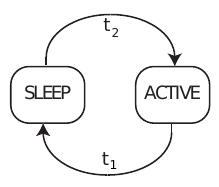
\includegraphics[width=0.2\textwidth]{./figures/task3.png}
  \end{tasknoinc}
  \begin{solutionnoinc}
    First we express the life time $L$ in terms of the maximal number of task executions $N_{\max }$ and period $T$ :
    \[
    L=N_{\max } \cdot T
    \]
    Then we set up an equation for the total energy that is consumed during the lifetime $L$ :
    \[
    \begin{aligned}
    E & =N_{\text {max }} \cdot\left(t_{\text {task }} \cdot P_{\text {active }}+\left(T-t_{\text {task }}\right) \cdot P_{\text {sleep }}\right) \\
    & =N_{\text {max }} \cdot\left(t_{\text {task }} \cdot P_{\text {active }}+\left(\frac{L}{N_{\text {max }}}-t_{\text {task }}\right) \cdot P_{\text {sleep }}\right) \\
    & =N_{\text {max }} \cdot\left(t_{\text {task }} \cdot P_{\text {active }}-t_{\text {task }} \cdot P_{\text {sleep }}\right)+L \cdot P_{\text {sleep }}
    \end{aligned}
    \]
    \end{solutionnoinc}
    \begin{solution}
    Solving for $N_{\max }$ results in:
    \[
    N_{\max }=\frac{E-L * P_{\text {sleep }}}{t_{\text {task }} *\left(P_{\text {active }}-P_{\text {sleep }}\right)}=4.87 * 10^6
    \]
    To support up to $N_{\max }$ executions, we can deduce that for $T$ the following must hold:
    \[
    T \geq \frac{L}{N_{\max }}=32.39 \mathrm{~s}
    \]
  \end{solution}
\end{frame}

\begin{frame}[allowframebreaks]{Task 3}{}
  \begin{solutionnoinc}
    Function $P(t)$ for schedules $\mathrm{S} 1$ and $\mathrm{S} 2$, for $t \in[0,800]$ is shown in the following diagram:
    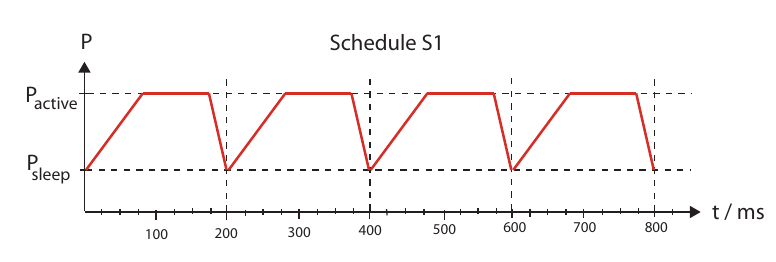
\includegraphics[width=\textwidth]{./figures/task3_2_1.png}
  \end{solutionnoinc}
  \begin{solution}
    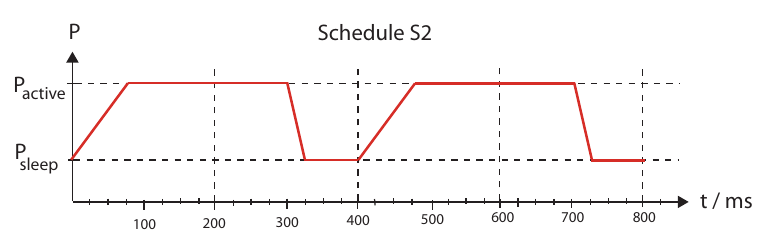
\includegraphics[width=\textwidth]{./figures/task3_2_2.png}
  \end{solution}
\end{frame}

\begin{frame}[allowframebreaks]{Task 3}{}
  \begin{solutionnoinc}
    The energy consumption of the Schedule $\mathrm{S} 2$, has a periodicity of $2 \cdot T$. Therefore we compute the energy difference for the first two periods and then average those values to get the average energy difference per period $T$. In the 1st period:
    \[
    \Delta E_1=E_{S 1}-E_{S 2}=t_1 \cdot \frac{P_{\text {sleep }}+P_{\text {active }}}{2}-t_1 \cdot P_{\text {active }}
    \]
    In the 2nd period:
    \[
    \Delta E_2=E_{S 1}-E_{S 2}=t_2 \cdot \frac{P_{\text {active }}+P_{\text {sleep }}}{2}-t_2 \cdot P_{\text {sleep }}
    \]
  \end{solutionnoinc}
  \begin{solution}
    On average, the energy difference per period between $\mathrm{S} 1$ and S2 is:
    \[
    \Delta E=\frac{\Delta E_1+\Delta E_2}{2}=\frac{\left(t_2-t_1\right)\left(P_{\text {active }}-P_{\text {sleep }}\right)}{4} \approx 13.875 \mu \mathrm{J}
    \]
  \end{solution}
\end{frame}

\begin{frame}[allowframebreaks]{Task 3}{}
  \begin{solutionnoinc}
    Function $P(t)$ for schedule S-OPT, for $t \in[0,800]$ is shown in the following diagram:
    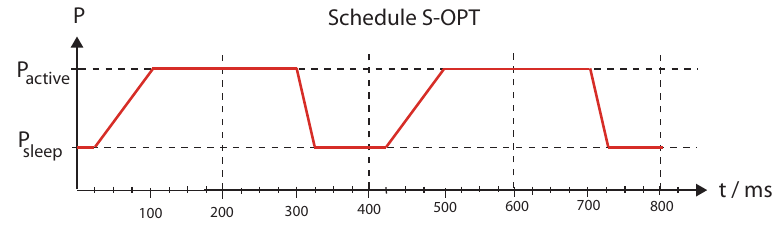
\includegraphics[width=\textwidth]{./figures/task3_3.png}
  \end{solutionnoinc}
  \begin{solutionnoinc}
    The energy consumption of the Schedule S-OPT, has a periodicity of $2 \cdot T$. Therefore we compute the energy difference for the first two periods and then average those values to get the average energy difference per period $T$. In the 1st period:
    \[
    \Delta E_1^{\prime}=t_1 \cdot \frac{P_{\text {active }}+P_{\text {sleep }}}{2}-t_1 \cdot P_{\text {sleep }}
    \]
    In the 2nd period:
    \[
    \Delta E_2^{\prime}=t_2 \cdot \frac{P_{\text {active }}+P_{\text {sleep }}}{2}-t_2 \cdot P_{\text {sleep }}
    \]
  \end{solutionnoinc}
  \begin{solution}
    On average, the energy difference per period between $\mathrm{S} 1$ and S-OPT is:
    \[
    \Delta E^{\prime}=\frac{\Delta E_1+\Delta E_2}{2}=\frac{\left(t_2+t_1\right)\left(P_{\text {active }}-P_{\text {sleep }}\right)}{4} \approx 27.75 \mu \mathrm{J}
    \]
  \end{solution}
\end{frame}
